\chapter{Descrizione dell'interfaccia}
\section{Prima esecuzione}
La prima volta che \xlogo\ viene lanciato (o se il file \texttt{.xlogo} è stato cancellato -Leggi la sezione  \ref{file_perso}-) una finestra di dialogo appare per chiedere di definire la lingua di utilizzo del programma stesso e dei programmi logo che con esso si realizzeranno.
\begin{center}
	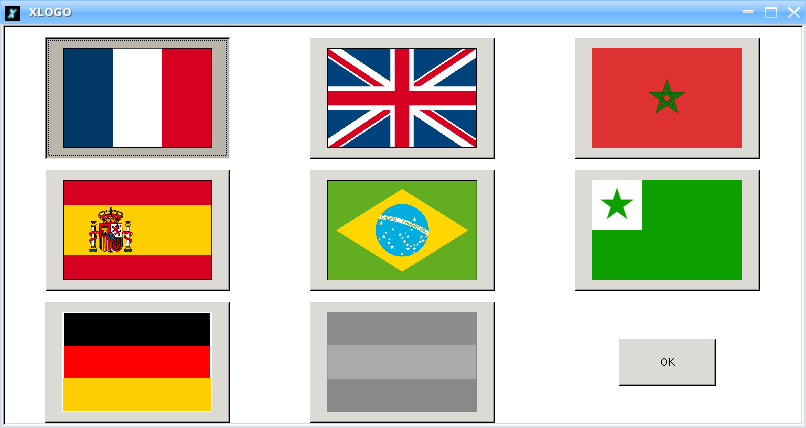
\includegraphics[scale=0.2]{pics/interface-CaptureLangue.png} 
\end{center}
La lingua predefinita può essere cambiata in qualsiasi momento nella finestra delle Preferenze (Sezione  \ref{general_tab}).
\section{La finestra principale}
\begin{center}
	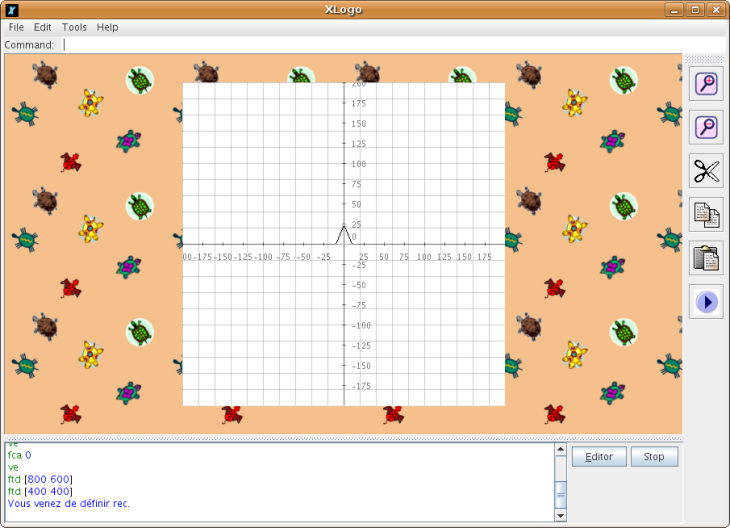
\includegraphics[  scale=0.4]{pics/interface-Capture.png} 
\end{center}

\begin{itemize}
	\item Nella parte superiore vi sono i menu usuali \textbf{File Modifica Strumenti e Aiuto}
	\item Appena al sotto è collocata la \textbf{linea di comando}, che permette alle istruzioni logo di essere eseguite.
	\item Nella parte centrale dello schermo vi è l'\textbf{area di disegno}. 
	\item Sulla destra dell'area di disegno una \textbf{barra degli strumenti} permette all'utente di eseguire numerose azioni:
	\begin{itemize}
		\item Ingrandire e rimpicciolire.
		\item Modifica (taglia/copia/incolla)
		\item Il bottone ``avvia'' lancia il comando principale definito nell'editor.
	\end{itemize}
	\item Nella parte inferiore vi è lo \textbf{storico dei comandi} che mostra tutti i comandi inseriti e la risposta associata dell'interprete. Per richiamare velocemente un comando che è stato già inserito ci sono due opzioni: o si clicca sul vecchio comando nello storico o si può cliccare sulla bassa di scorrimento finché il vecchio comando appare nell'elenco. La barra di scorrimento permette di navigare attraverso tutti i comandi inseriti (molto pratico). 
	\item Alla destra dello storico ci sono due bottoni: \textbf{STOP} e \textbf{EDITOR}. 
	\begin{itemize}
		\item Il bottone STOP interrompe l'esecuzione del programma logo.
		\item Il bottone EDITOR apre la l'editor delle procedure.\\ 
	\end{itemize}
\end{itemize}
\section{L'editor delle procedure}
\begin{center}
	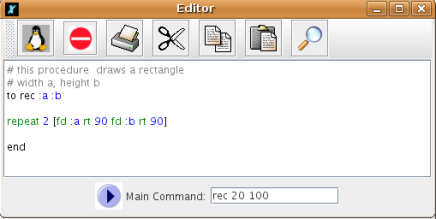
\includegraphics[scale=0.4]{pics/interface-CaptureEditor.png}
\end{center}
Esistono tre modi per aprire l'editor:\\
\begin{itemize}
	\item Digita \texttt{ed} sulla linea di comando nella parte superiore dello schermo. L'editor si apre mostrando tutte le procedure già definite. Se si vuole modificare una o più procedure specifiche digitare:\\
	\texttt{ed {[}procedura\_1 procedura\_2 $\ldots$]}
	\item Premi il bottone Editor nello schermo principale. 
	\item Premi i tasti Alt+E sulla tastiera. 
\end{itemize}
I seguenti sono i vari bottoni che si trovano nell'editor:\\

\begin{longtable}{cm{12cm}}
	\includegraphics*[scale=1]{pics/interface-turtle.png} &
	Salva i cambiamenti effettuati nell'editor e ne chiude la finestra. È questo il bottone che occorre premere ogni volta per inserire le nuove procedure digitate. È possibile anche premere i tasti Alt+Q sulla tastiera.\\
	\includegraphics*[scale=1]{pics/interface-quit.png}&
	Chiude la finestra dell'editor senza salvare i cambiamenti effettuati. È possibile anche premere i tasti Alt+C sulla tastiera.\\
	\includegraphics*[scale=1]{pics/interface-fileprint.png}&
	Stampa il contenuto dell'editor.\\
	\includegraphics*[scale=1]{pics/interface-editcopy.png}&
	Copia il testo selezionato negli appunti.\\
	\includegraphics*[scale=1]{pics/interface-editcut.png}&
	Taglia il testo selezionato negli appunti.\\
	\includegraphics*[scale=1]{pics/interface-editpaste.png}&
	Incolla il testo selezionato negli appunti.\\
	\includegraphics*[scale=1]{pics/interface-chercher.png}&
	Apri un riquadro per Cercare/Sostituire del testo nell'editor.\\
\end{longtable}
\begin{center}
	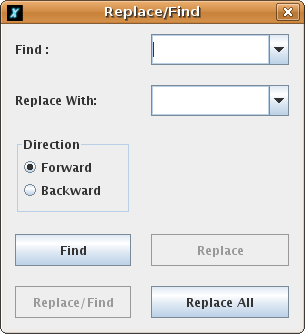
\includegraphics[scale=0.4]{pics/interface-CaptureFind.png}
\end{center}
\vspace{0.5cm}

\includegraphics{pics/interface-play.png}
Nella farte inferiore dell'editor un campo di testo permette di definire un comando principale. Questo comando è l'istruzione generale che lancia il programma logo. Può essere acceduta tramite il bottone ``Avvia'' dalla barra degli strumenti della finestra principale. Questo comando viene salvato e caricato insieme al programma logo (con estensione \texttt{.lgo}) viene salvato tramite l'editor. \\ \\
\textbf{\begin{Large}IMPORTANTE\end{Large}} \\
\begin{itemize}
	\item Da notare che cliccando sul bottone di chiusura della finestra dell'editor (x), l'editor non si chiuderà! Solo uno dei due bottoni principale consente la chiusura dell'editor. 
	\item Per cancellare una o più procedure occorre usare le primitive \texttt{CancProc} e \texttt{CancTutte} nella linea di comando, o usare il gestore delle procedure che si trova nel menu Strumenti.
\end{itemize}
\section{Chiudere \xlogo}
Per chiudere \xlogo, si può scegliere \textbf{File - Abbandona} nella barra dei menu, o cliccare sul bottone di chiusura nella barra del titolo della finestra. una finestra di dialogo chiede quindi di confermare la chiusura del programma.\\
\textbf{Nota per l'ambiente Mac}. In ambiente Mac è preferibile non utilizzare la funzione di chiusura dell'applicazione presente di default nella barra dei menu fornita da Mac OS ma utilizzare i due metodi esposti al paragrafo precedente.
\begin{center}
	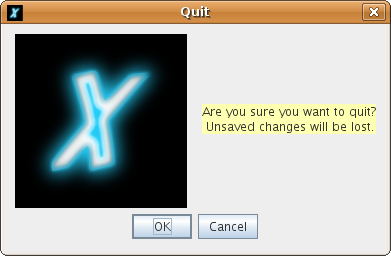
\includegraphics[scale=0.4]{pics/interface-CaptureQuit.png}
\end{center}





\chapter{Opzioni del menu}

\section{Menu ``File''}
\begin{itemize}
	\item \textbf{File$\to$Nuovo}: crea un nuovo ambiente di lavoro, cancella tutte le procedure e variabili.
	\item \textbf{File$\to$Apri}: apre un file logo precedentemente salvato.
	\begin{center}
		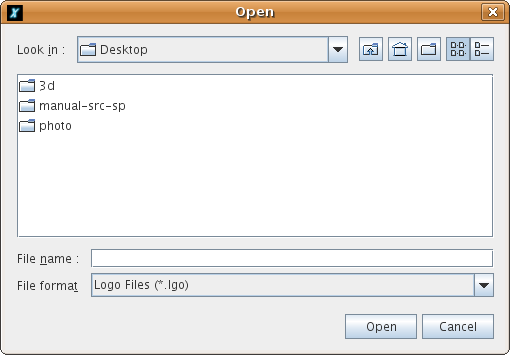
\includegraphics[scale=0.4]{pics/interface-CaptureOpen.png}
	\end{center}
	\vspace{0.25cm}
	\item \textbf{File$\to$Registra come\textellipsis} salva le procedure correnti con un nome diverso.
	\begin{center}
		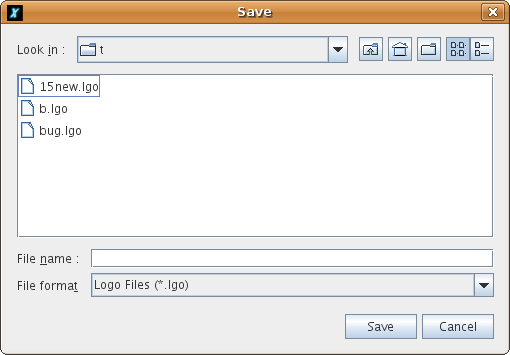
\includegraphics[scale=0.4]{pics/interface-CaptureSave.png}
	\end{center}
	\vspace{0.25cm}
	\item \textbf{File$\to$Registra}: salva le procedure nel file corrente
	\item \textbf{File$\to$Cattura$\to$Registra come\textellipsis}: permette di salvare l'immagine dell'area di disegno in formato jpeg o png. Se vuoi registrare solo una parte dell'immagine puopi definire un'area rettangolare trascinando il mouse sull'area di disegno.
	\vspace{0.25cm}
	\item \textbf{File$\to$Cattura$\to$Stampa\textellipsis}: permette di stampare l'immagine o parte di essa.
	\item \textbf{File$\to$Cattura$\to$Copia Appunti}: copia l'immagine o parte di essa negli appunti di sistema. Funziona in ambiente Windows e Mac OS, non in Linux (gli appunti hanno un comportamento diverso).
	\item \textbf{File$\to$Testo$\to$Registra come\textellipsis (formato RTF)}: registra lo storico dei comandi in formato RTF (preservando colori e formati).
	\item \textbf{File$\to$Abbandona}: esce da \xlogo.
\end{itemize}

\section{Menu ``Modifica''}
\begin{itemize}
	\item \textbf{Modifica$\to$Copia}: copia il testo selezionato negli appunti.
	\item \textbf{Modifica$\to$Taglia}: taglia il testo selezionato negli appunti.
	\item \textbf{Modifica$\to$Incolla}: Incolla il testo degli appunti nella linea di comando.
	\item \textbf{Modifica$\to$Selezina tutto}: Seleziona tutto il testo nella linea di comando.
\end{itemize}

\section{Menu ``Strumenti''}
\begin{itemize}
	\item \textbf{Strumenti$\to$Colore Penna}: permette di impostare il colore della penna della tartaruga scegliendo da una gamma di colori. E' anche accessibile dal comando \texttt{ImpCP}.
	\begin{center}
		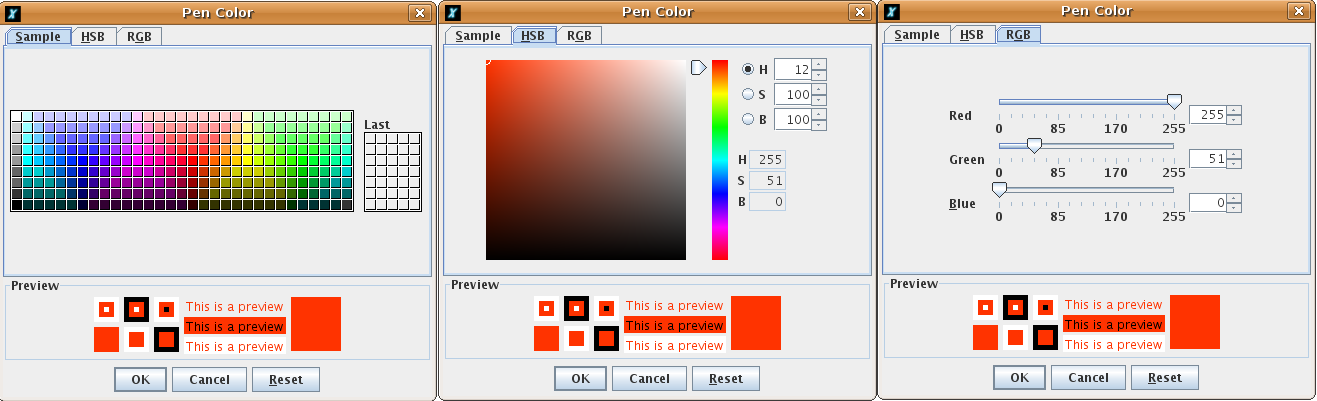
\includegraphics[scale=0.3]{pics/interface-CaptureColor.png}
	\end{center}
	\vspace{0.25cm}
	\item \textbf{Strumenti$\to$Colore Sfondo}: imposta il colore dello sfondo dell'area di disegno, anche accessibile tramite la primitiva \texttt{ImpCS}.
	\item \textbf{Strumenti$\to$File di partenza}: permette di definire il percorso ad un file di avvio. Tutte le procedure contenute in questo file .lgo diventeranno quindi ``pseudo-primitive'' nel linguaggio \xlogo. Non possono essere modificate dall'utente. Puoi quindi definire primitive personalizzate.
	\begin{center}
		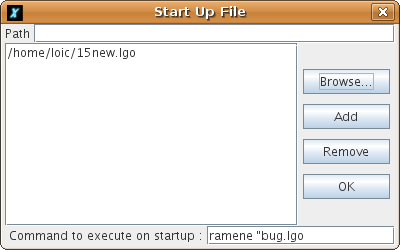
\includegraphics[scale=0.4]{pics/interface-CaptureStart.png}
	\end{center}
	\vspace{0.25cm}
	\item \textbf{Strumenti$\to$Traduttore primitive}: permette di tradurre il codice di \xlogo\ da una lingua all'altra. E' molto utile quando si vuole tradurre un esempio scritto in un'altra lingua.
	\begin{center}
		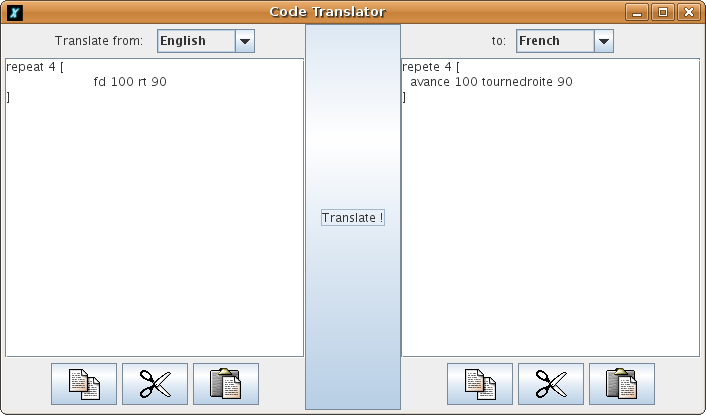
\includegraphics[scale=0.4]{pics/interface-CaptureTranslator.png}
	\end{center}
	\vspace{0.25cm}
	\item \textbf{Strumenti$\to$Gestione procedure}: apre una finestra che permette di cancellare le procedure definite nell'editor. Puoi anche definire l'ordine di comparsa delle procedure nell'editor.
	\begin{center}
		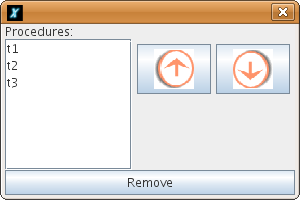
\includegraphics[scale=0.4]{pics/interface-CaptureProcedure.png}
	\end{center}
	\vspace{0.25cm}
	\item \textbf{Strumenti$\to$Preferenze}: apre una finestra che permette di configurare diversi aspetti di \xlogo:
	\begin{itemize}
		\label{general_tab}
		\item \textbf{Tab generale} 
		\begin{itemize}
			\item \textbf{Lingua}: permette di scegliere una diversa lingua, nta che anche le primitive vengono tradotte nella lingua scelta.
			\item \textbf{Aspetto}: permette di impostare l'aspetto di \xlogo tra ``Metal'', ``Nativo  Java'' e ``Motif''.
			\item \textbf{Velocità della tartaruga}: Se preferisci osservare i movimenti della tartaruga puoi rallentarla usando la slitta.
			\end{itemize}. 
			\begin{center}
				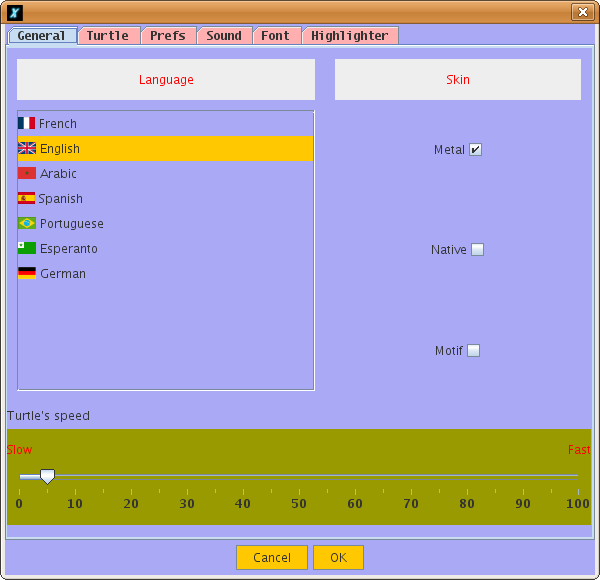
\includegraphics[scale=0.3]{pics/interface-CapturePref1.png}
				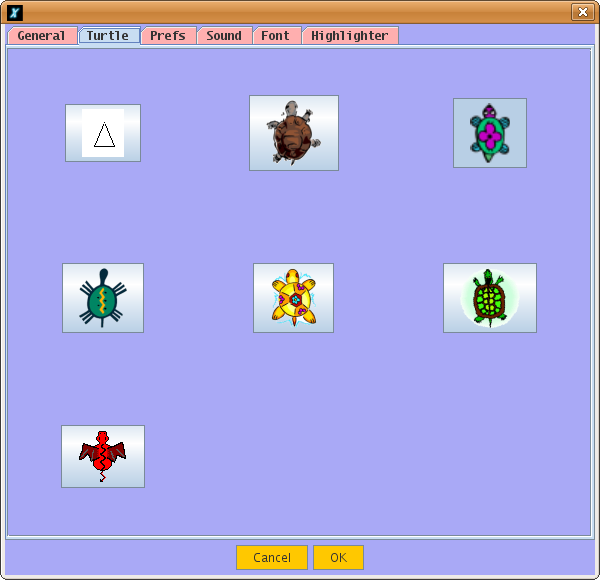
\includegraphics[scale=0.3]{pics/interface-CapturePref2.png}
			\end{center}
			\vspace{0.25cm}
%			\item \textbf{Tab tartaruga}: Puoi scegliere l'immagine della tartaruga che preferisci.
%			\begin{center}
%				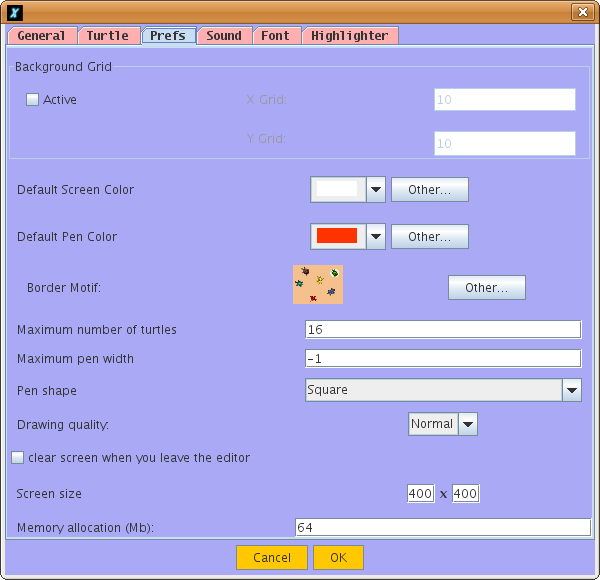
\includegraphics[scale=0.4]{pics/interface-CapturePref3.png}
%			\end{center}
			\item \textbf{Tab opzioni}: Vi sono molte opzioni:
			\begin{itemize}
				\item \textbf{Griglia di sfondo}: Puoi scegliere di disegnare una griglia sullo sfondo dell'area di disegno. Puoi definire l'ampiezza e l'altezza del quadrato della griglia ed il suo colore.
				\item \textbf{Assi sullo sfondo dello schermo}: Puoi disegnare l'asse orizzontale e/o verticale sullo sfondo dell'area di disegno. Puoi definire la distanza tra due divisioni dell'asse ed il colore dell'asse.
				\item \textbf{Colore dello schermo}: Puoi definire un colore dello schermo preimpostato.
				\item \textbf{Colore della penna}: Puoi definire un colore preimpostato della penna.
				\item \textbf{Motivo del bordo}: Puoi scegliere il tuo motivo per l'area esterna a quella del disegno.
				\begin{center}
					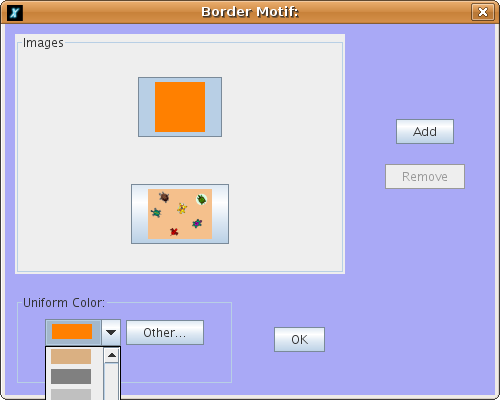
\includegraphics[scale=0.4]{pics/interface-CaptureBorder.png}
				\end{center}
				\item \textbf{Massimo numero di tartarughe}
				\item \textbf{Massima ampiezza della penna}: Puoi scegliere la massima ampiezza della penna permessa (-1 disabilita un limite massimo).
				\item \textbf{Forma della punta della penna}
				\item \textbf{Qualità della traccia da disegno}: Puoi scegliere l'accuratezza della traccia del disegno. In alta qualità gli angoli saranno arrotondati ma la velocità di disegno diminuisce.
				\item \textbf{Pulisci lo schermo quando si chiude l'editor}: alla chiusura dell'editor l'area di disegno viene ripulita o meno.
				\item \textbf{Cancella le variabili quando chiudi l'editor}: alla chiusura dell'editor tutte le variabili vengono cancellate.
				\item \textbf{Dimensione dell'area di disegno}: dimensioni in pixel. Attenzione, aree di disegno più grandi richiedono maggiore memoria.
				\item \textbf{Memoria allocata a XLogo (MB)}: Aree di disegno grandi o programmi ricorsivi hanno bisogno di maggiore memoria di quella predefinita. La modifica di questo parametro richiede di riavviare \xlogo. \textcolor{red}{Attenzione}, non aumentare troppo questo parametro poiché potrebbe rallentare considerevolmente il computer.
				\item \textbf{Numero porta TCP}: Puoi modificare la porta preimpostata TCP per le comunicazioni di rete (cfr. pagina \pageref{network})
			\end{itemize}
			\begin{center}
				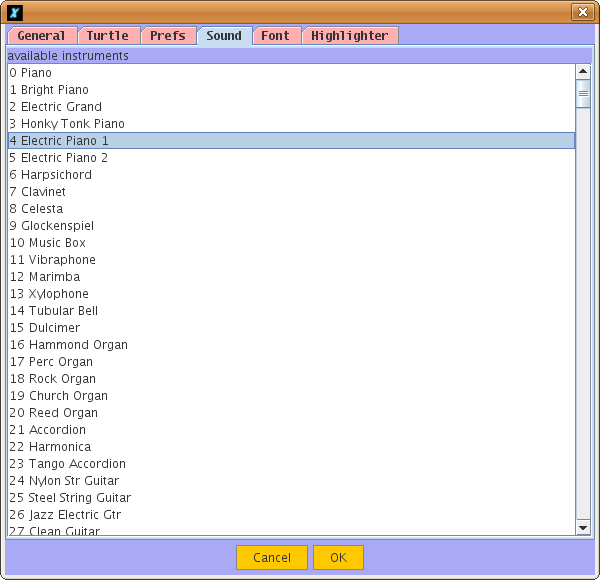
\includegraphics[scale=0.4]{pics/interface-CapturePref4.png}
			\end{center}
			\vspace{0.25cm}
			\item \textbf{Tab Suono}: Puoi scegliere lo strumento musicale per l'interfaccia MIDI. Se l'elenco degli strumenti è vuoto dai uno sguardo alla sezione FAQ del manuale alla fine del manuale. Questa funzione può anche essere acceduta dalla primitiva \texttt{ImpostaStrumento}.
			\begin{center}
				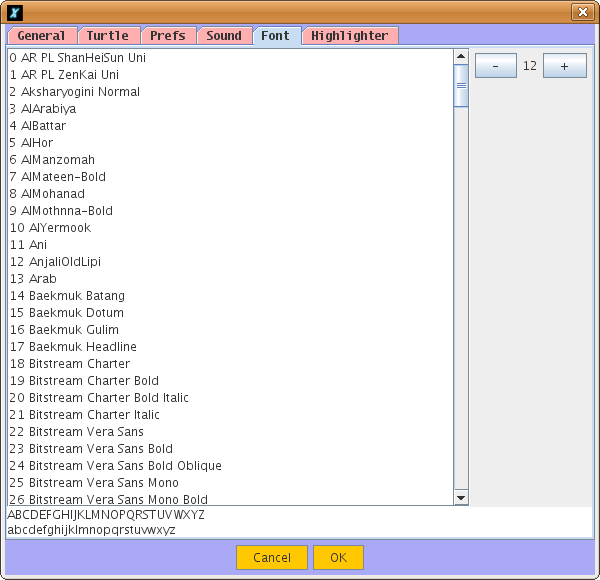
\includegraphics[scale=0.4]{pics/interface-CapturePref5.png}
			\end{center}
			\vspace{0.25cm}
			\item \textbf{Tab Font}: Puoi scegliere il font per l'interfaccia.
			\begin{center}
				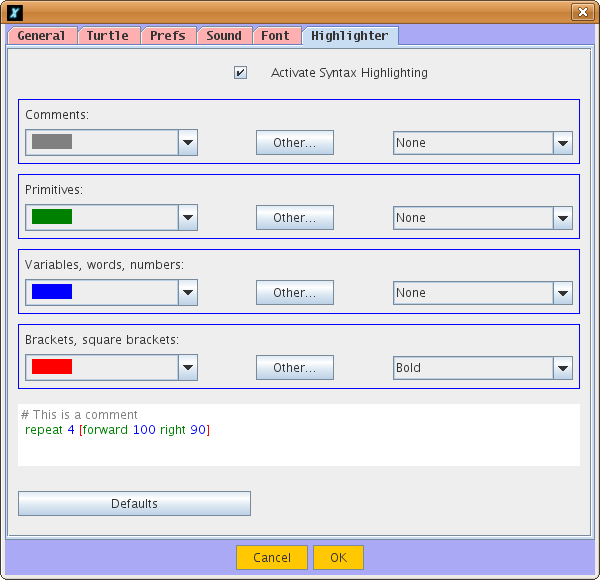
\includegraphics[scale=0.4]{pics/interface-CapturePref6.png}
			\end{center}
			\vspace{0.25cm}
			\item \textbf{Tab Colorazione}: Puoi scegliere di attivare la colorazione sintattica e definire i colori che preferisci.
		\end{itemize}
	\end{itemize}
	\section{Menu ``Aiuto''}
	\begin{itemize}
		\item \textbf{Aiuto$\to$Manuale on-line}: Visualizza il manuale di riferimento per \xlogo, accessibile su Internet.
		\vspace{0.25cm}
		\item \textbf{Aiuto$\to$Licenze}: visualizza la licenza GPL sotto la quale viene distribuito \xlogo.
		\begin{center}
			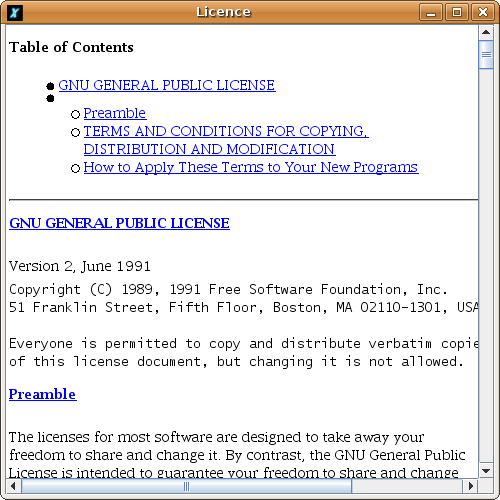
\includegraphics[scale=0.4]{pics/interface-CaptureLicence.png}
		\end{center}
		\vspace{0.25cm}
		\item \textbf{Aiuto$\to$Traduzione della licenza}: visualizza una traduzione della licenza, anche se non ha carattere di ufficialità.
		\item \textbf{Aiuto$\to$Traduci \xlogo}: questa finestra di dialogo permette di consultare, modificare, completare le traduzioni di \xlogo di tutte le lingue (primitive e messaggi).
		\begin{center}
			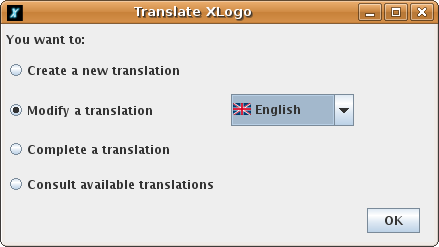
\includegraphics[scale=0.4]{pics/interface-CaptureXLogoTranslate1.png}
			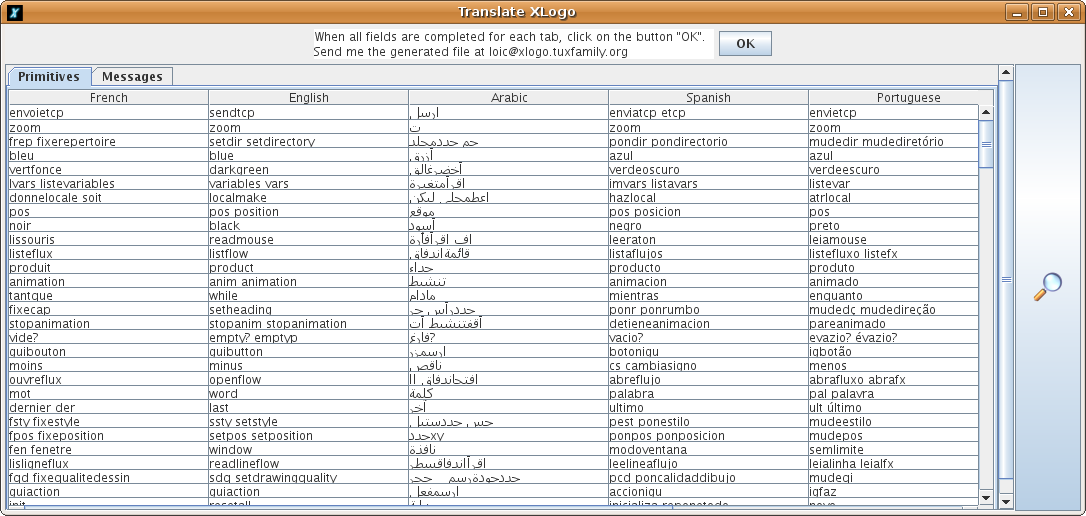
\includegraphics[scale=0.4]{pics/interface-CaptureXLogoTranslate2.png}
		\end{center}
		\vspace{0.25cm}
		Altrimenti puoi creare una traduzione per una nuova lingua. In tutti i casi mandami il file generato a \texttt{loic@xlogo.tuxfamily.org}
		\item \textbf{Menu -- > Informazioni su \xlogo}: la classica finestra e xlogo.tuxfamily.org per i tuoi segnalibri !! o:) 
		\begin{center}
			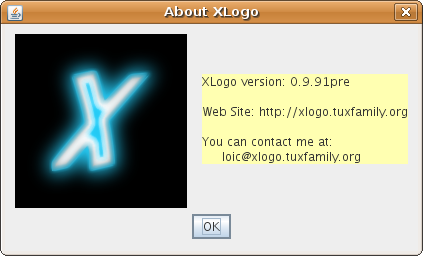
\includegraphics[scale=0.6]{pics/interface-CaptureAbout.png}
		\end{center}
		\vspace{0.25cm}
	\end{itemize}
